\section{Main Experimental Insights}    \label{sec:insights}
% Main Experimental Insights

%% Discussion of sources of error
While the presented model-based control strategy works well enough to be useful for some robotic control tasks, there are several shortcomings that severely limit its accuracy and precision, thereby prohibiting its use in more high-fidelity control applications. A weakness of any purely model-based control approach is the unavoidable inaccuracies introduced by various modeling assumptions. Notably, in our model of FREEs, we assume them to be perfectly cylindrical, which is clearly violated whenever a FREE is bent, buckled, or kinked. We also assume that the elastomeric force component is a function of deformation only, when other models suggest it may be more accurately represented as a function of pressure and deformation \cite{sedal2017constitutive}.

%% Proposed improvements: Feedback is still needed to account for errors in modeling, sysid, etc.
Incorporating a feedback term into our control law in addition to the model-based feed-forward term could make up for many of the shortcomings of our model. This could be done by incorporating a corrective PID control term at each time step. The pressure input at the $k^{th}$ discrete time step would then be equal to
\begin{align}
    \p_k = \p + \delta \p_k
\end{align}
where $\p$ is the minimizer of \eqref{eq:QP} for a given $\x_\tx{des}$, and $\delta \p_k$ is the iteratively calculated solution to 
\begin{align}
    0 = \J_x^T \delta \p_k - K \e_k - I \sum_0^{k} \e_k - D (\e_k - \e_{k-1})
\end{align}
and
\begin{align}
    \e_k = \x_k - \x_\tx{des}
\end{align}

\Dan{This is just a quick and dirty summary of what I have in mind for the feedback part. We should discuss this part before more detail added...}

In future experiments we plan to incorporate this added feedback term into our controller and compare its performance against the purely feed-forward controller presented in section \ref{sec:technical-approach}.

%% figure: photo of the full rig with motion capture and pressure regulators visible
\begin{figure}
    \centering
    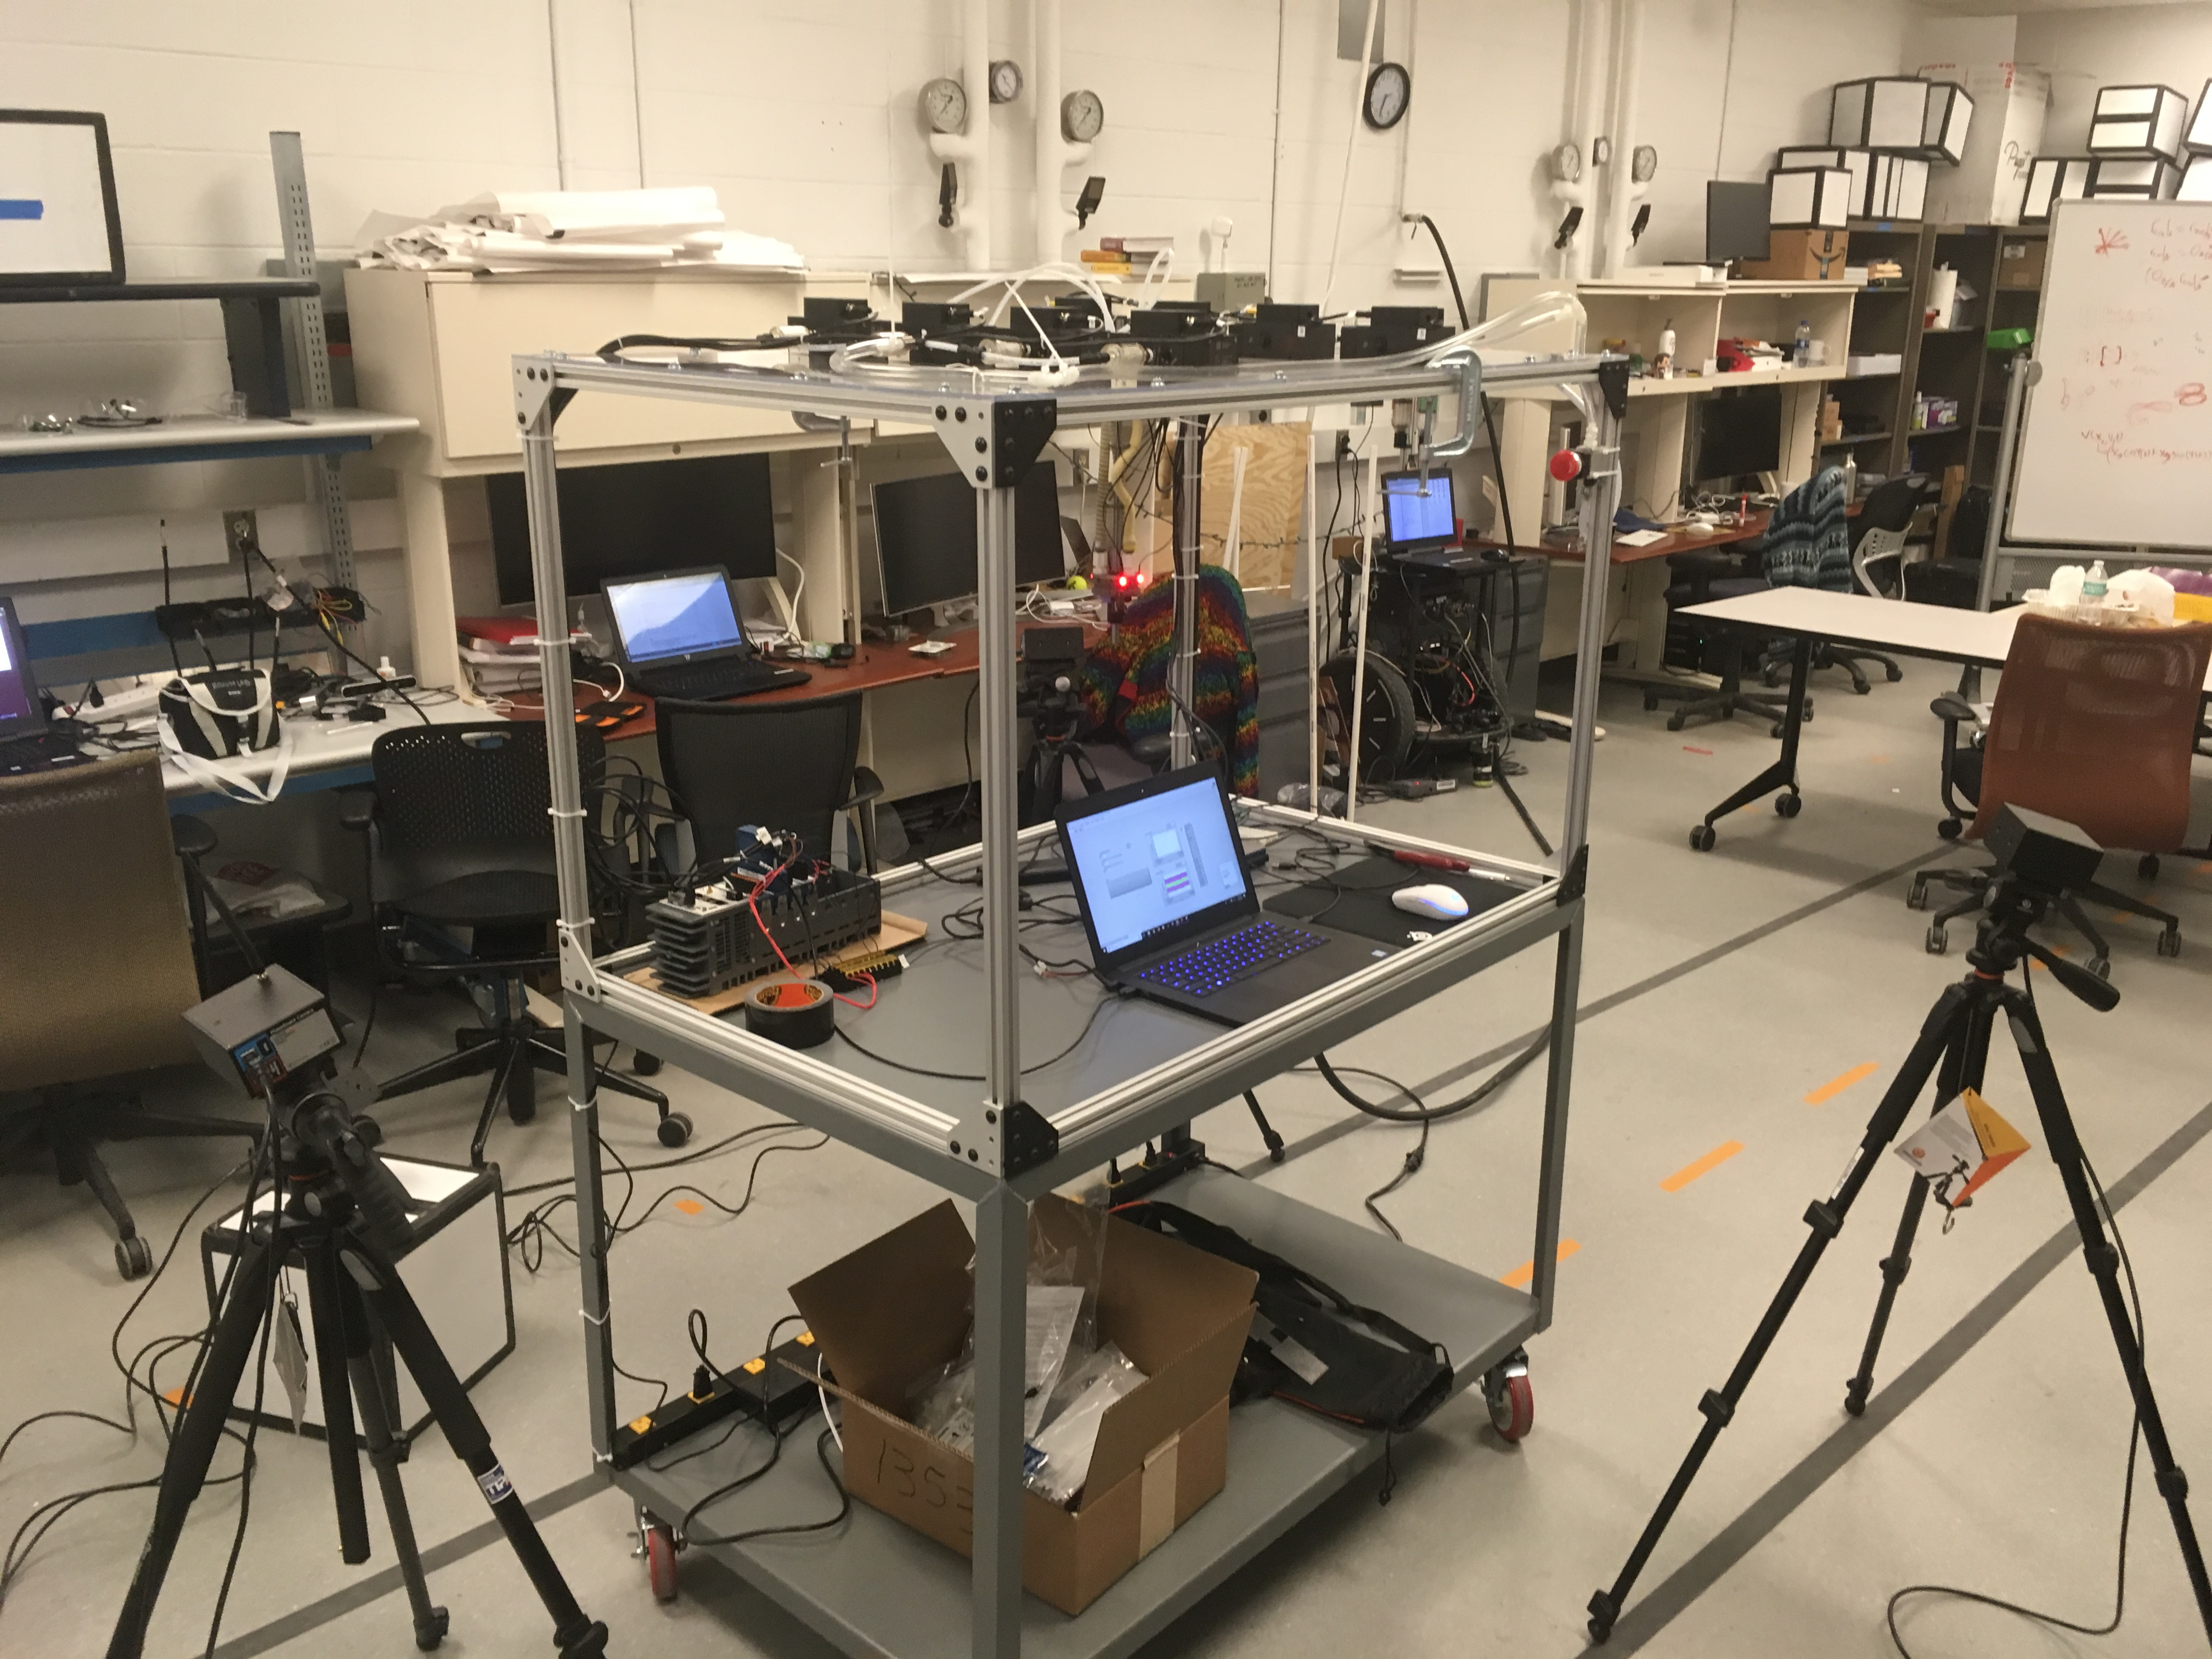
\includegraphics[width=0.5\linewidth]{figures/fullRig.JPG}
    \caption{Real photo would be less cluttered and have things labeled, i.e. Daq, regulators, mocap cameras, etc. \Dan{This doesn't actually belong here, but I feel like there should be an image that shows the entire test set up with the motion capture cameras and pressure regulators labeled. Maybe not necessary since this is just and abstract but I'm leaving it here to get your thoughts on it.}}
    \label{fig:fullRig}
\end{figure}




%Another source of error comes from limitations imposed by hardware. The actuators we use are hand-made in the lab, so unmodified fabrication errors are ubiquitous. And our ability to control pressure and measure displacements is limited by the accuracy of our pressure regulators and motion capture system respectively 